\chapter{Algoritmos sustracción del fondo}

\section{Introducción}


Esta sección hace una presentación de los algoritmos que emplean modelos estadísticos para describir el segundo plano de una secuencia. Se detalla el modelo de Mixtura de Gaussianas propuesto por \textit{Zivkovic y Heidjen} \cite{zivkovic_efficient_2006}, y la mejora propuesta por \textit{Zezhi Chen} \cite{chen_vehicle_2012}. Se describe además el modelo no-parametrico de \textit{Elgammal} \cite{elgammal_nonparametricmodel_2000}.




\section{Modelo General}

La idea en general del proceso de sustracción de fondo es modelar cada uno de los píxeles de una escena mediante una función de densidad de probabilidad. Se fundamenta, en la suposición que las imágenes de una escena sin objetos en circulación, tienen un comportamiento regular que puede ser descrito por un modelo estadístico. Un evento podría ser detectado, identificando las partes de la imagen que no se ajustan con el modelo que describe el fondo. El píxel de una imagen nueva sólo se considera parte del fondo, si su valor queda completamente descrito por la función de densidad de probabilidad. 


El valor de intensidad en el tiempo de un píxel (o en el transcurso de una secuencia) es utilizado para construir una función de densidad de probabilidad, la cual corresponde al modelo estadístico que describe el comportamiento del píxel. El modelo, es determinado por una combinación lineal de un conjunto de distribuciones Gaussianas, y por su parte, cada componente es caracterizado por un grupo de parámetros, que identifica los elementos que emergen durante el avance de las imágenes.

\begin{figure}[h!]
  \centering
      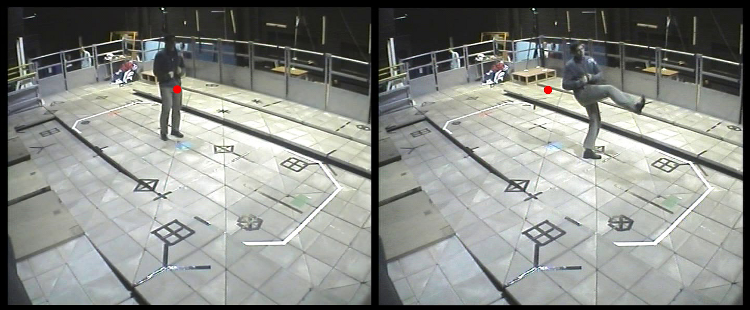
\includegraphics[scale=0.5]{img/figura_3_1}
  \caption[Imágenes 570, 610 de secuencia ``\textit{Kick Camera 3 Person 4}'']{Imágenes 570 y 610 de la secuencia MuHAVI-MAS ``\textit{Kick Camera 3 Person 4}''. El punto en rojo señala la posición de un píxel en dos eventos diferentes}
\label{posicion_340_160}
\end{figure}

\begin{figure}[h!]
  \centering
      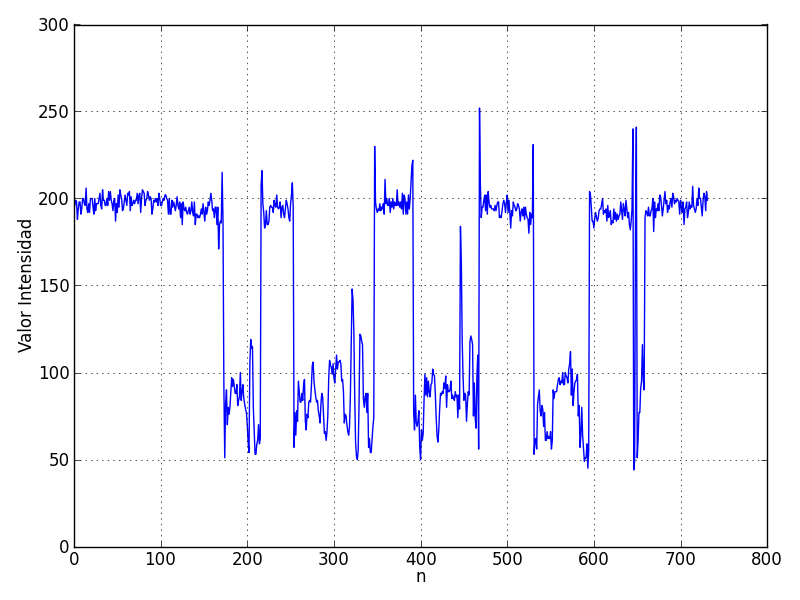
\includegraphics[scale=0.5]{img/figura_3_2}
  \caption[Cambios de intensidad en el tiempo del valor de un pixel ]{Cambios del valor de intensidad de un color en la secuencia completa.}
\label{intensidad_340_160}
\end{figure}


La separación de píxeles entre elementos del fondo y otros objetos, puede ser explicado en forma muy sencilla, con las dos imágenes de la figura \ref{posicion_340_160} tomadas de la secuencia MuHAVI \textit{``Kick Camera 3 Person 4''}\cite{singh_muhavi_2010}. Estas imágenes señalan el estado de un píxel (punto en rojo) en dos instantes diferentes. La primera imagen, el píxel forma parte del actor (\textit{foreground}) en medio del escenario y su valor es determinado por los colores de la vestimenta. La siguiente imagen el actor ha cambiado su posición, y en este caso el valor del píxel queda definido por los colores del escenario (\textit{background}). La figura \ref{intensidad_340_160} representa el cambio de intensidad (para un color) de la secuencia completa (730 imágenes) producido por los varios cruces del actor en medio del escenario. Por razones computacionales, se asume que los valores de intensidad de los tres componentes (valores de píxel azul, verde y rojo) tienen la misma varianza\cite{zivkovic_efficient_2006}, de esta manera la matriz de covarianza queda definida como una matriz identidad multiplicado por este valor de varianza.

\begin{figure}[h!]
  \centering
      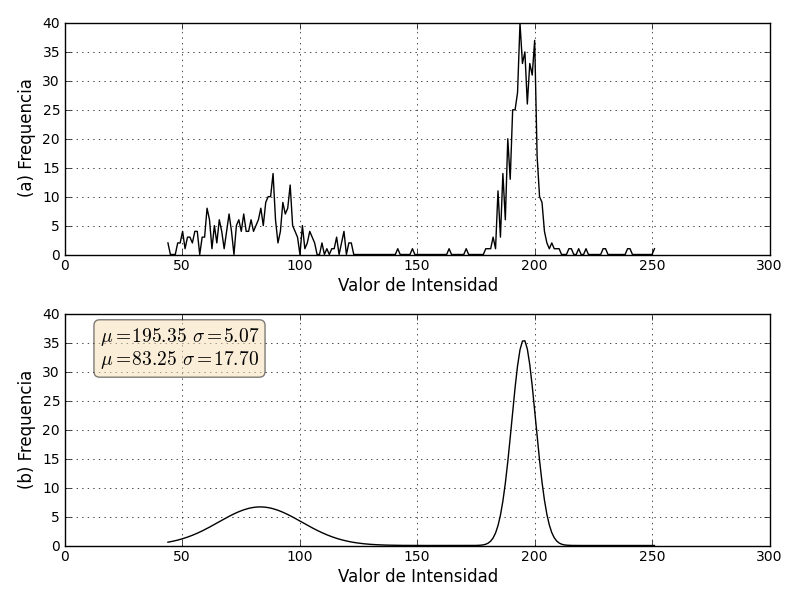
\includegraphics[scale=0.75]{img/histograma_pixel_340_160_3_2}
  \caption[Histograma secuencia completa ``\textit{Kick Camera 3 Person 4}'']{Histograma secuencia completa ``\textit{Kick Camera 3 Person 4}''}
\label{histograma}
\end{figure}

Una rápida observación de la figura (\ref{intensidad_340_160}) muestra que los valores asociados al escenario son más constante (o menor dispersión) que los valores del actor cuando atraviesa este píxel. Esto también se puede apreciar en el modelo de la secuencia completa que describe el histograma de la figura (~\ref{histograma})(a). En esta imagen se pueden distinguir dos curvas bien definidas, el fondo de imagen y el el actor en movimiento. La mixtura en este ejemplo se construye ajustando la función de densidad a dos distribuciones Gaussianas, figura (\ref{histograma})(b). De esta manera, el modelo que describe este píxel en particular, queda completamente definido por una composición de dos funciones Gaussianas. Se observa además en esta figura, que la imagen de fondo se puede asociar con la componente de menor valor de varianza, debido principalmente a la menor dispersión de valores del fondo. Sin embargo, el menor valor de frecuencia se puede relacionar con el actor en movimiento, por el menor tiempo que éste se cruza en el escenario. 

De esta forma el algoritmo puede hacer una separación entre \textit{foreground} y \textit{background}  cuando la componente Gaussiana que describe algún píxel no se ajuste a la distribución con menor varianza, considerando este elemento parte de un objeto en movimiento. No obstante, si este mismo objeto queda estático por un tiempo considerable, su distribución Gaussiana comenzará a mostrar un varianza similar a la varianza del fondo, en ese momento el píxel se considera parte del fondo.




\begin{figure}[h!]
  \centering
      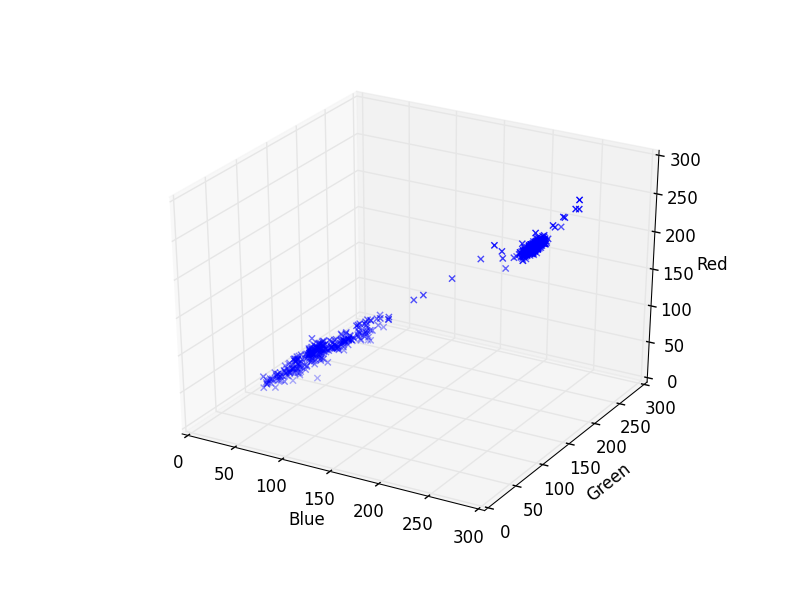
\includegraphics[scale=0.75]{img/scatter_pt_340_160_3D_Blue_Green_Red}
  \caption[Gráfico dispersión 3D secuencia completa ``\textit{Kick Camera 3 Person 4}'']{Gráfico de dispersión en secuencia ``\textit{Kick Camera 3 Person 4}'' que muestra la nube de puntos relacionados con el escenario y el actor en movimiento.}
\label{scatter_3D}
\end{figure}

\begin{figure}[h!]
  \centering
      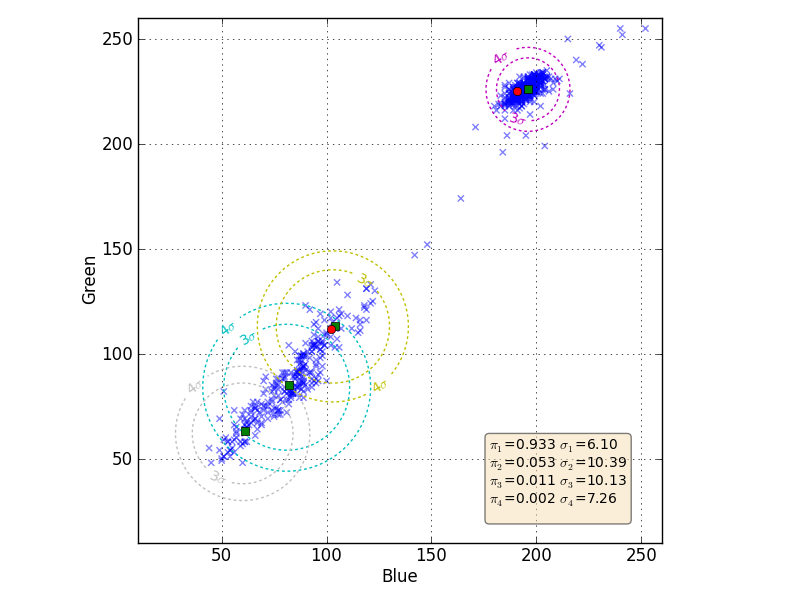
\includegraphics[scale=0.75]{img/scatter_pt_340_160_isotropic_Blue_Green}
  \caption[Gráfico dispersión 2D secuencia completa ``\textit{Kick Camera 3 Person 4}'']{Gráfico de dispersión secuencia ``\textit{Kick Camera 3 Person 4}'', que muestra dos \textit{cluster} bien definidos}
\label{scatter_2D}
\end{figure}

Los gráficos de las figuras \ref{scatter_3D} y \ref{scatter_2D} sirven de ejemplo para entender el funcionamiento y procedimiento de actualización de los parámetros, para cada uno de los componentes Gaussianos definidos en el algoritmo. Estas figuras son gráficas de dispersión del valor de un píxel (azul, verde y rojo) en toda la secuencia ``\textit{Kick Camera 3 Person 4}'', tomado del ejemplo en la figura \ref{posicion_340_160}. La dispersión de puntos en la gráfica \ref{scatter_3D} conforma principalmente dos nubes o \textit{clusters} que se asocian con los dos elementos principales de la secuencia: el escenario y las acciones del actor. El \textit{cluster} más compacto de puntos, localizado en el rango 150-250 de los tres ejes de colores, resume los diferentes tiempos que el píxel fue parte del escenario, mientras el otro \textit{cluster} localizado en la parte inferior refleja la cantidad de veces que el píxel formo parte del actor durante sus movimientos.  

Durante la ejecución del algoritmo, los componentes Gaussianos de un píxel se van creando o suprimiendo en tiempo real, dependiendo de los valores de una nueva entrada y el tiempo de permanencia de estos valores, en alguno de los clusters de la secuencia. Los valores del píxel presentan un comportamiento dinámico, estos se pueden mover entre \textit{clusters} o bien se mantiene en uno de ellos, en relación directa con los eventos en la secuencia. Se aprovecha esta división de \textit{clusters} para hacer la separación entre \textit{background} y \textit{foregorund}. La figura \ref{scatter_2D} muestra la dispersión de valores entre los colores azul y verde. En esta gráfica se han destacado cuatro \textit{clusters} (componentes Gaussianos) definidos por el algoritmo, en el instante que el actor estaba posicionado sobre el píxel. los puntos en rojo señalan la posición del pixel en los dos instantes indicados por la figura \ref{posicion_340_160}. Cada una de estos componentes tiene un factor de ponderación $\pi_k$ que indica en cierta forma el tiempo de permanencia del píxel en la nube de puntos. Este factor de ponderación es incrementado en la medida que el valor del píxel se mantenga dentro de un cierto margen (de uno de los componentes), determinado por la distancia de Mahalanobis, de los clusters. En este ejemplo, para discriminar que el píxel es parte del actor, el algoritmo calcula la distancia del pixel a los diferentes ``centroides'' (media) de los clusters. La distancia menor a tres veces la varianza asocia el punto con ese \textit{cluster} específico y por lo tanto el píxel queda determinado por la característica de ese cluster, es decir, si el cluster en particular tiene un factor de ponderación más alto que todos los demas, ese cluster es \textit{background} y por ende el píxel. En caso contrario, el píxel que pertenece a un cluster con factor de ponderación inferior, pertenece algún objeto en movimiento y en consecuencia el píxel también.  




\section{Mixtura de distribuciones Gaussianas - GMM}


La superposición de distribuciones Gaussianas que describen el comportamiento de un pixel, se define en la ecuación \eqref{eq:mixturegaussians}. Esta es una sumatoria de \textit{``K''} componentes Gaussianos $\mathcal{N}( x | \mu_k , \Sigma_k)$, cada uno ponderado por un factor multiplicativo $\pi_k$, la cual establece una función de densidad de probabilidad general para el píxel $p(x)$. El factor de ponderación $\pi_k$ es el grado de influencia de cada componente, en el comportamiento global del píxel que esta siendo modelado. Los valores de ponderación pueden ser interpretados, como probabilidades de ocurrencias de las diferentes clases, \textit{Background} y \textit{Foreground}, representadas por los diferentes componentes Gaussianos; por ejemplo, $\pi_1$ podría representar la probabilidad que un píxel sea la imagen de fondo. La suma total de los factores $\pi_k$ es 1, indicado en la ecuación \eqref{eq:mixturefactor}. 

\begin{equation} \label{eq:mixturegaussians}
p(x) = \sum_{k=1}^{K} \pi_k \mathcal{N}( x | \mu_k , \Sigma_k)
\end{equation}

\begin{equation} \label{eq:mixturefactor}
\sum_{k=1}^{K} \pi_k = 1
\end{equation}


Una de las principales tareas del algoritmo que implementa mixtura de Gaussianas, es mantener actualizado los $K$ valores estimados de media ($\mu_1, ..., \mu_k$),  covarianza ($\Sigma_1, ..., \Sigma_k$) y el factor de ponderación ($\pi_1, ..., \pi_k$), por cada píxel de una nueva imagen. Se utilizan los valores de intensidad en el espacio de colores RGB, para construir la mixtura de componentes Gaussianas de un píxel.

La estimación de los parámetros $\vec{\theta} = \{\pi_1,..,\pi_k, \mu_1,..,\mu_k,\Sigma_1,..,\Sigma_k \} $ de las distintas mixturas se realiza mediante el método de Máxima Verosimilitud (\textit{Maximum Likelihood Estimate - MLE}). De esta manera, los parámetros estimados por máxima verosimilitud de un conjunto $t$ de muestras $\mathcal{X} = \{\vec{x}^{(1)}, ..., \vec{x}^{(t)}\}$, quedan determinados por la ecuación (~\ref{eq:maxima_verosimilutd}). Una explicación bien detallada de estimación mediante el método de máxima verosimilitud se puede ver en el capítulo 3 de la referencia \cite{duda_pattern_2000}.

\begin{equation} \label{eq:maxima_verosimilutd}
\hat{\vec{\theta}} = arg \max_{\vec{\theta}}  (\log p(\mathcal{X};\vec{\theta}))
\end{equation}

 
Debido a la dificultad de encontrar una solución analítica de \textit{MLE}, se emplea una aproximación numérica iterativa para maximizar la función de verosimilitud.  El algoritmo de esperanza-maximización (EM) \cite{dempster_maximum_1977} se usa para encontrar soluciones de máxima verosimilitudes. Este es un procedimiento iterativo que busca un máximo local de la función log-verosimilitud. Este algoritmo es fácil de implementar, sin embargo una de sus limitaciones es la posibilidad de converger en un máximo local muy malo debido que no fue inicializado apropiadamente.


\subsection{Actualización parametros del Algoritmo}

Esta parte describe el método de actualización recursivo que se utiliza en la estimación de los parámetros ($\mu_k$, $\Sigma_k$, $\pi_k$) de cada componente Gaussiano, establecido por \textit{Zivkovic y Heidjen} \cite{zivkovic_efficient_2006}. Por razones computacionales las matrices de covarianza son consideradas Isotrópicas, es decir la matriz de identidad multiplicado por un único valor de varianza.

El modelo del fondo es estimado desde un conjunto de entrenamiento ``$X$'', el cual mantiene una historia específica de muestras por cada píxel. Este conjunto es constantemente actualizado con nuevas muestras, para adecuarse a los posibles cambios que puedan producirse. Y simultáneamente va descartando las muestras más antiguas. Un periodo de adaptación ``$T$'' (100 cuadros) es elegido para mantener la historia más reciente del fondo, y en el instante ``$t$'' se tiene el conjunto de entrenamiento $\mathcal{X_T} = \{x^{(t)}, ..., x^{(t-T)}\}$, desde el cual se estima la función de densidad del fondo.

La parte central del algoritmo, consiste en actualizar constantemente los parámetros $\vec{\theta}$ de las distribuciones Gaussianas, que describen el estado de cada píxel en un momento determinado. Las ecuaciones recursivas para estimar los parámetros de una muestra nueva $x^{(t)}$ en tiempo $t$ se presentan a continuación:


\begin{equation} \label{eq:mixturefactor_update}
\hat{\pi}_k \leftarrow  \hat{\pi}_k + \alpha(o^{(t)}_k - \hat{\pi}_k) - \alpha C_T
\end{equation}
\begin{equation} \label{eq:mixturemu_update}
\hat{\vec{\mu}}_k \leftarrow \hat{\vec{\mu}}_k + o^{(t)}_k (\alpha/\hat{\pi}_k) \vec{\delta}_k
\end{equation}
\begin{equation} \label{eq:mixturesigma_update}
\hat{\sigma}^2_k \leftarrow \hat{\sigma}^2_k + o^{(t)}_k (\alpha/\hat{\pi}_k) (\vec{\delta}^T_k \vec{\delta}_k - \hat{\sigma}^2_k)
\end{equation}
\begin{equation} \label{eq:mahalanobis_distance}
D^{2}_{k}(\vec{x}^{(t)})=\vec{\delta}^T\vec{\delta}_k/\hat{\sigma}^{2}_k
\end{equation}

\[
\vec{\delta}_k = \vec{x}^{(t)} - \hat{\vec{\mu}}_k
\]


El factor constante $\alpha$ define una curva de decaimiento exponencial para limitar la influencia de los datos más antiguos. Se usa esta constante como reemplazo de $T$ mencionado anteriormente, relacionando ambas constante por la siguiente relación: $\alpha=1/T$. 

El algoritmo mantiene un conjunto dinámico de componentes por cada píxel, esto significa que el número de componentes del modelo es diferente en periodos distintos de la secuencia. Se determina que una nueva muestra es cercana con algunos de los componentes si la distancia de \textit{Mahalanobis} \eqref{eq:mahalanobis_distance} es por ejemplo, menor que tres. Fijando el valor del \textit{ownership} $o^{(t)}_k$ en uno si la muestra es cercana y en cero para el caso contrario. Si la muestra no es cercana a alguno de los componentes ($o^{(t)}_k=0$), se crea uno nuevo con los siguientes valores por defecto $\pi_{k+1} = \alpha$, $\hat{\vec{\mu}}_{k+1}=\vec{x}^{(t)}$ y $\hat{\sigma}_{k+1}=\sigma_0$, con $\sigma_0$ un valor de inicialización de la varianza fijado en el algoritmo.

Este algoritmo representa también los diferentes elementos que surgen en la secuencia, como un conjunto de \textit{clusters} en tiempo real. Un nuevo objeto que ingresa en la secuencia se caracteriza por un \textit{cluster} adicional con un valor de ponderación $\pi_k$ muy inferior a los otros componentes. 

Para determinar el píxel como una imagen de fondo, se ordena los factores de ponderación en forma descendente, y los $B$ \textit{clusters} con mayor ponderación se aproximan al modelo del fondo como se indica en la siguiente ecuación.

\begin{equation} \label{eq:clusters}
B=arg \max_{b}  (\sum_{k=1}^{b} \hat{\pi}_k > (1 - c_f))
\end{equation}

El parámetro $c_f$ es un criterio de medición que indica la cantidad de los datos que pueden ser considerados objetos de \textit{foreground} sin la influencia del modelo de \textit{background}. De esta forma si un nuevo objeto se mantiene estático durante algún tiempo, este será presentado como un \textit{cluster} adicional, y su factor de ponderación $\pi_{k+1}$ será incrementado en la medida que se mantenga estático. Sí se mantiene lo suficiente, y el factor $\pi_{k+1}$ supera $c_f$, entonces este objeto puede ser considerado parte del fondo.


\section{Modelo Mixtura de Gaussianas auto-adaptativo}

Este método se origina en un contexto de vigilancia de tráfico en ciudad. Es el resultado de un sistema de detección y clasificación automática de vehículos \cite{chen_vehicle_2012}, que utiliza una variante del método de mixtura de Gaussianas\cite{zivkovic_efficient_2006} para hacer separación entre vehículos en circulación y su pista. La modificación propuesta aborda el problema de cambios bruscos en la iluminación, que podrían transformar todo el segundo plano (\textit{background}) de la imagen en primer plano (\textit{foreground}). Además la tasa normal de aprendizaje se transforma en una tasa dinámica y en tiempo real de aprendizaje, se intenta con esta modificación obtener una tasa que se adapte en forma dinámica a los cambios de iluminación. También se utiliza como método de procesamiento previo un filtro espacial y temporal\cite{chen_background_2009} para compensar las alteraciones producidas por vibraciones de las camaras. Finalmente para afrontar el problema de cambios en iluminación local, como sombras y reflexiones de luz, modifican un algoritmo de extracción de sombras \cite{horprasert_astatistical_1999} para incorporar el factor de iluminación global.


\subsection{Factor de iluminación global}
En \cite{chen_self-adaptive_2011} se menciona el modelo de detección de cambio invariante a iluminación (\textit{ICDM}), al proceso que determina el factor de cambio de iluminación global.  Éste es un procedimiento que realiza el cociente uno a uno entre un conjunto $s$ de pixeles de una imagen de entrada ($i_c$) y su imagen de referencia ($i_r$). El factor de iluminación global $g$ se determina como la mediana de todas las divisiones resultantes, ``\textit{Median of Quotient (MofQ)}''.

\begin{equation} \label{eq:mofq}
g = \median_{(s \in S)}  \left(\frac{i_{r,s}}{i_{c,s}}\right)
\end{equation}

Se define además un contador ``$c_k$'' por cada componente Gaussiano en la mixtura. Este contador se utiliza para mantener un registro de cuantos puntos han contribuido en la estimación de parámetros de cada Gaussiana, cada vez que los parámetros de un componente Gaussiano es actualizado, el contador también es actualizado. En caso que un nuevo componente se agrega a la mixtura este contador es inicializado a uno. 

El factor de aprendizaje $\alpha$ es usado como base para construir un nuevo factor de aprendizaje $\beta$, el cual utiliza el contador de componentes Gaussianas mencionado anteriormente. Las nuevas ecuaciones de actualización de parámetros se detallan a continuación:


\begin{equation} \label{eq:sagmm_betha}
\beta_k = \alpha(h + c_k)/c_k
\end{equation}

\begin{equation} \label{eq:sagmm_mu}
\hat{\vec{\mu}}_k \leftarrow \hat{\vec{\mu}}_k + o^{(t)}_k (\beta/\hat{\pi}_k) \vec{\delta}_k
\end{equation}

\begin{equation} \label{eq:sagmm_sigma}
\hat{\sigma}^2_k \leftarrow \hat{\sigma}^2_k + o^{(t)}_k (\beta/\hat{\pi}_k) (\vec{\delta}^T_k \vec{\delta}_k - \hat{\sigma}^2_k)
\end{equation}

\begin{equation} \label{eq:sagmm_ck}
c_k \leftarrow c_k + 1
\end{equation}

\begin{equation} \label{eq:sagmm_delta}
\hat{\vec{\delta}}_k = g \bullet \vec{x}^{t} - \hat{\vec{\mu}}_k
\end{equation}

Si el valor de un pixel de la imagen de fondo varia muy rápidamente, el valor del contador $c_k$ para ese píxel no será muy grnade, por lo que el valor de $\beta$ aumentará. Actualizando de esta manera el fondo más rápidamente. Por otra parte si el fondo  es muy estable el contador, el valor se $\beta$ se aproximara a $\alpha$. También se observa que la distancia de Mahalanobis es balanceada por el factor de cambio de iluminación global $g$.


\subsection{Filtro espacial y temporal}
Este filtro que prepara la imagen antes de ser procesada por el método modificado de mixturas. Realiza un suavizado de cada componente espectral. En una imagen se habla de dominio espacial para referirse a los píxeles localizados en la matriz de valora. El dominio espectral y dominio temporal.

\begin{equation} \label{eq:sagmm_filter}
K_{h_s,h_s} = \frac{C}{h_s h_t} k \left( {\| \frac{x^s}{h_s} \|}^2 \right) k \left( {\| \frac{x^t}{h_t} \|}^2 \right)
\end{equation}

$C$ es una constante de normalización, $x^s$ es la parte espacial y $x^t$ la parte temporal, $k(x)$ es un perfil común de kernel (Gaussiano) usado en ambos dominios, temporal y espacial. Las variable $h_s$ y $h_t$ son el ancho de banda de los kernels. 


\begin{figure}[h!]
\centering
\fbox{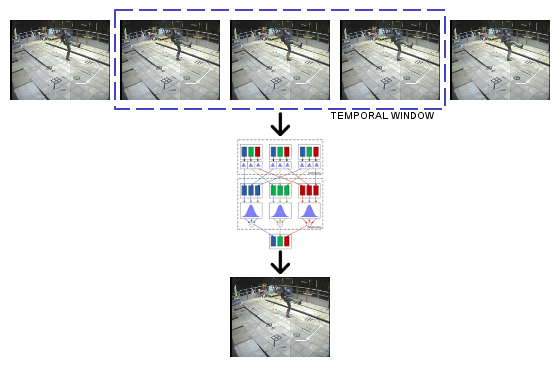
\includegraphics[scale=0.5]{img/Spatio_Temporal_Filter_Example}}
\caption[Procesamiento temporal de tres imágenes]{Procesamiento temporal de tres imágenes de una secuencia.}
\label{fig:spatio_temporal_filter_example}
\end{figure}


La figura \ref{fig:spatio_temporal_filter_example} es un ejemplo del funcionamiento de este filtro. Se define una ventana temporal que define el número de imágenes que serán procesadas simultáneamente por este filtro. La entrada del filtro es el número de imágenes que mantiene la ventana temporal y su salida es una imagen preparada que será la nueva entrada del algoritmo. Esta ventana puede ser visualizada como un marco que se desliza sobre la secuencia y entrega una procesada como salida.

\begin{figure}[h!]
\centering
%\subfigure{%\documentclass{article}
\documentclass[preview]{standalone}
%\usepackage{tikz}
\usepackage{pgfplots}
%\usepackage{subfigure}

\begin{document}

\newcommand\gauss[2]{1/(#2*sqrt(2*pi))*exp(-((x-#1)^2)/(2*#2^2))} 
\tikzstyle{place}=[circle,draw=blue!50,fill=blue!20,thick]


\begin{tikzpicture}[scale=0.5,cube/.style={very thin,black}]
    %\draw[step=1cm,gray,very thin] (-2,-2) grid (24,24);

    \node[inner sep=0cm] (gaussian) at (2.75,7.5)
        {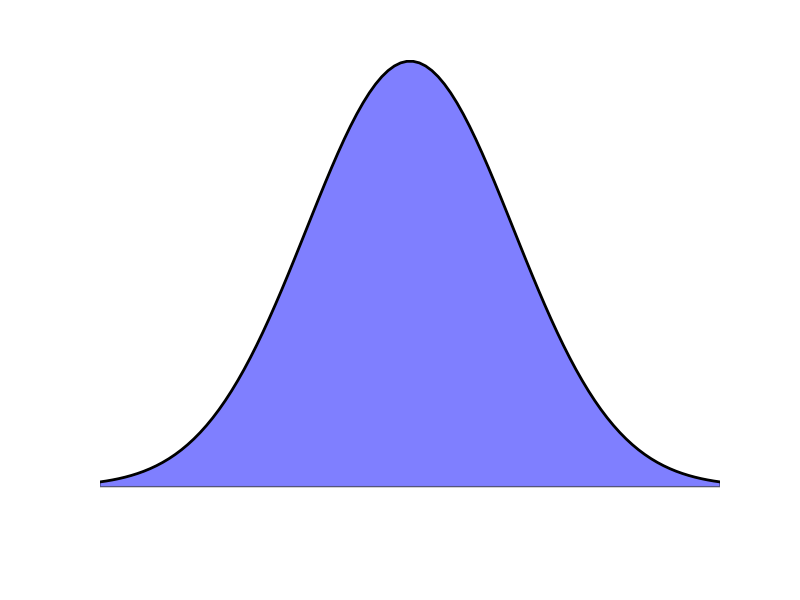
\includegraphics[width=.14\textwidth]{gaussian.png}};
    \node[inner sep=0cm] (gaussian) at (6.75,7.5)
        {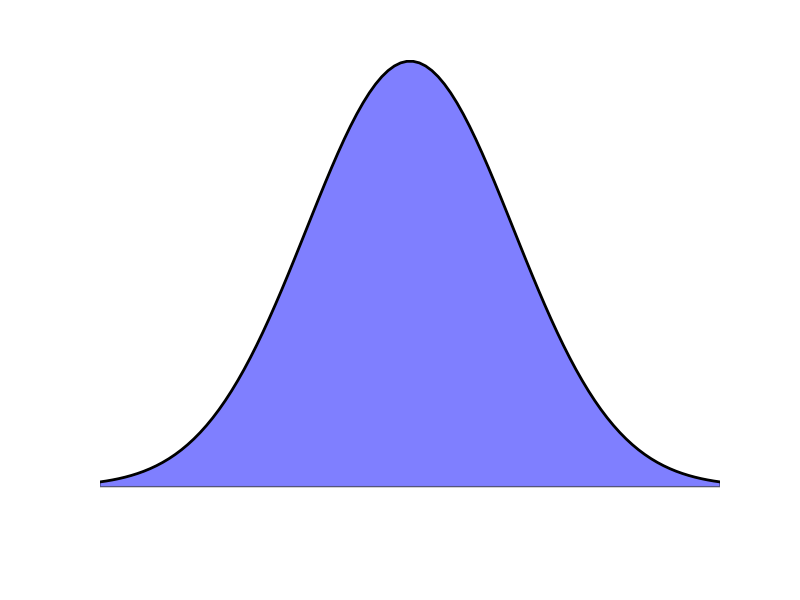
\includegraphics[width=.14\textwidth]{gaussian.png}};
    \node[inner sep=0cm] (gaussian) at (10.75,7.5)
        {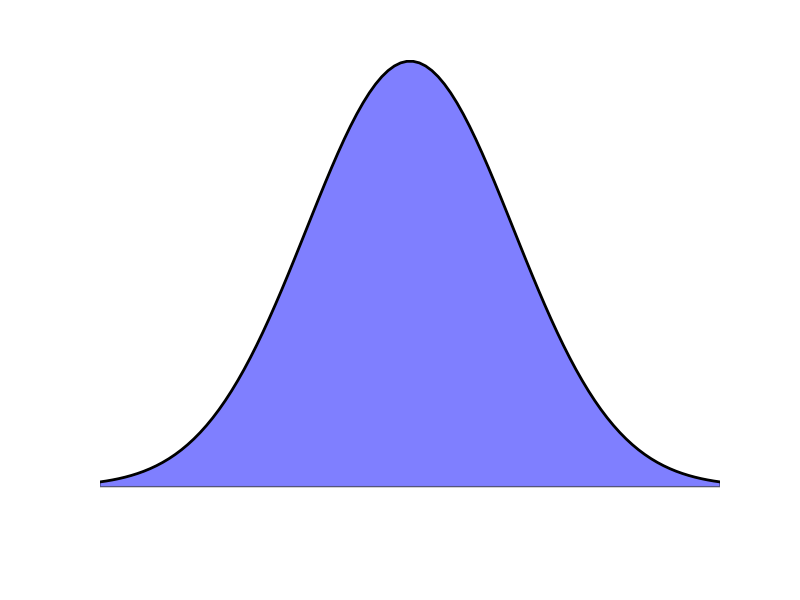
\includegraphics[width=.14\textwidth]{gaussian.png}};

    \node[inner sep=0cm] (gaussian) at (1.5,17.5)
        {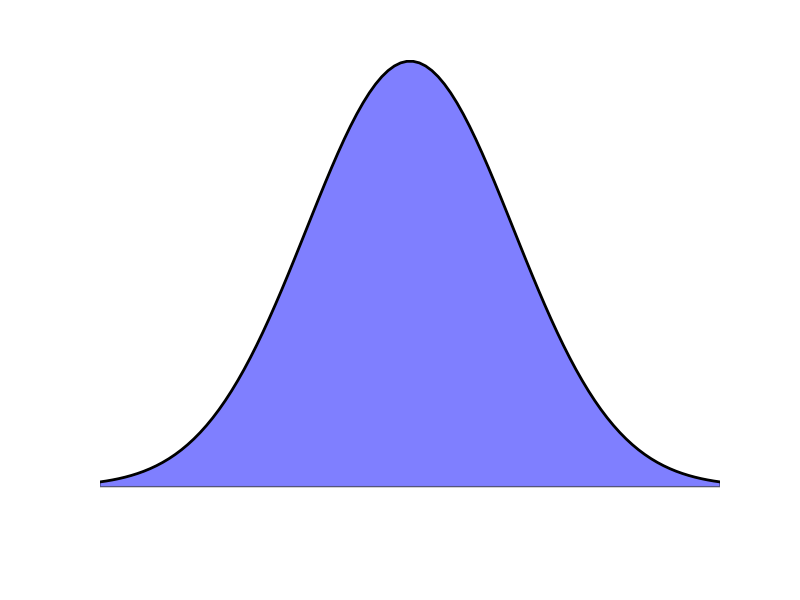
\includegraphics[width=.05\textwidth]{gaussian.png}};
    \node[inner sep=0cm] (gaussian) at (2.5,17.5)
        {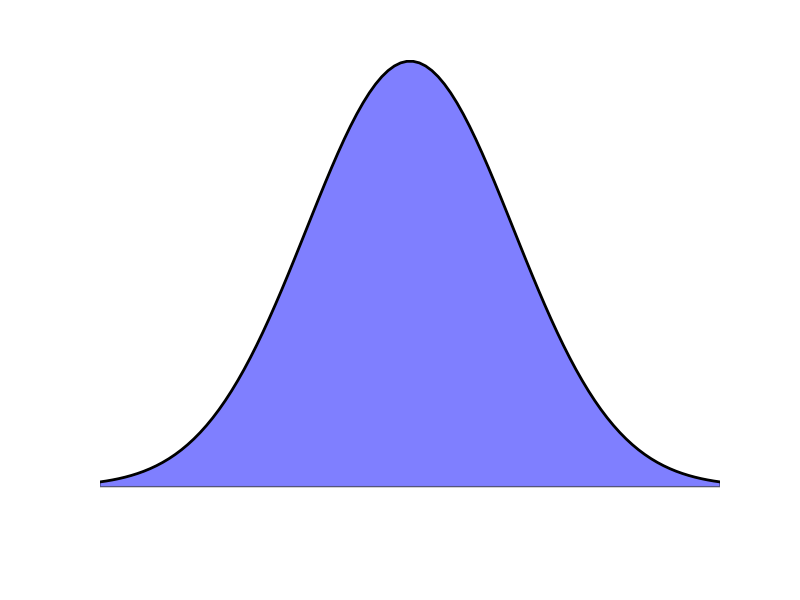
\includegraphics[width=.05\textwidth]{gaussian.png}};
    \node[inner sep=0cm] (gaussian) at (3.5,17.5)
        {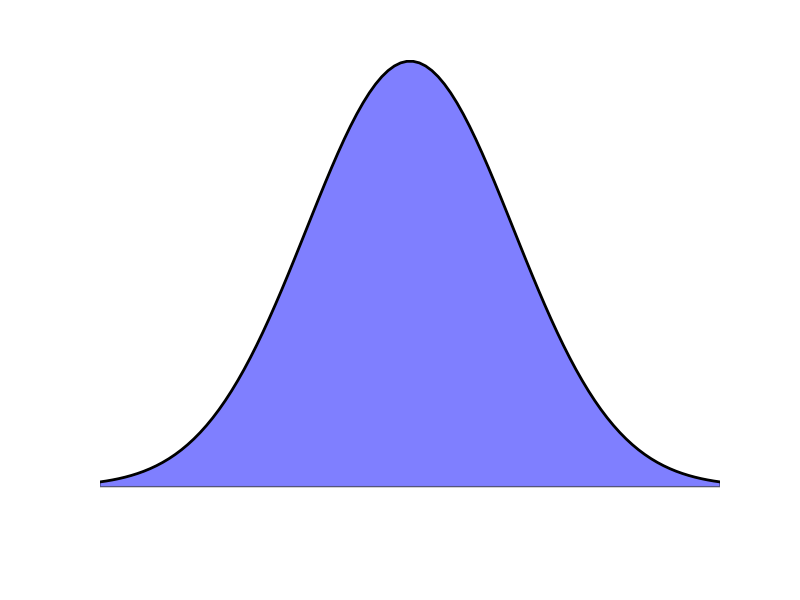
\includegraphics[width=.05\textwidth]{gaussian.png}};

    \node[inner sep=0cm] (gaussian) at (5.5,17.5)
        {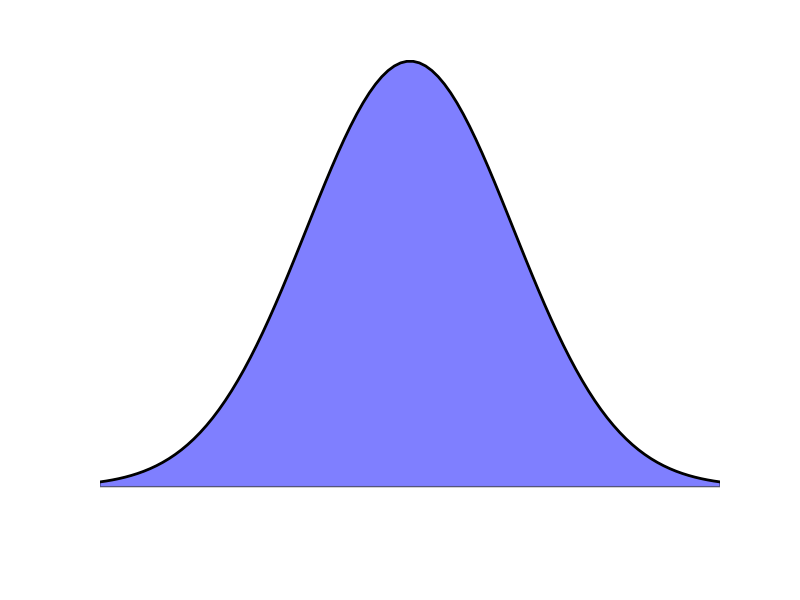
\includegraphics[width=.05\textwidth]{gaussian.png}};
    \node[inner sep=0cm] (gaussian) at (6.5,17.5)
        {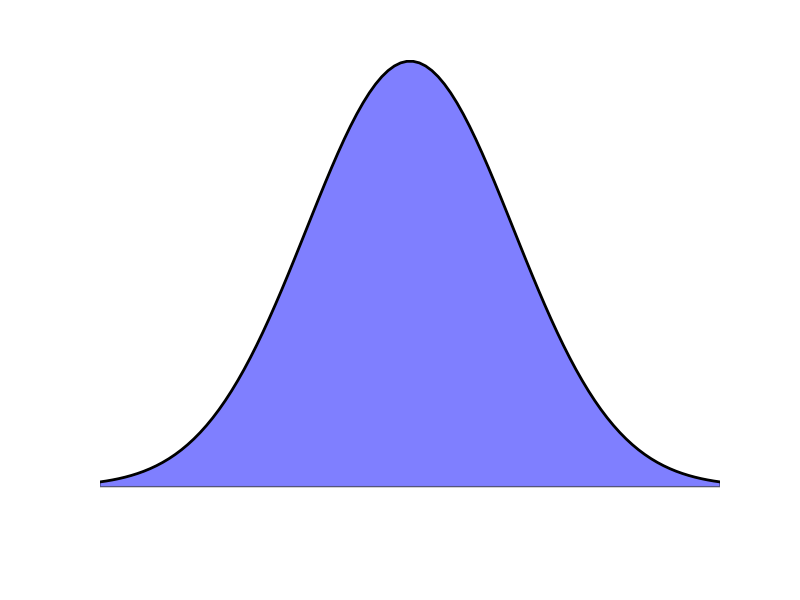
\includegraphics[width=.05\textwidth]{gaussian.png}};
    \node[inner sep=0cm] (gaussian) at (7.5,17.5)
        {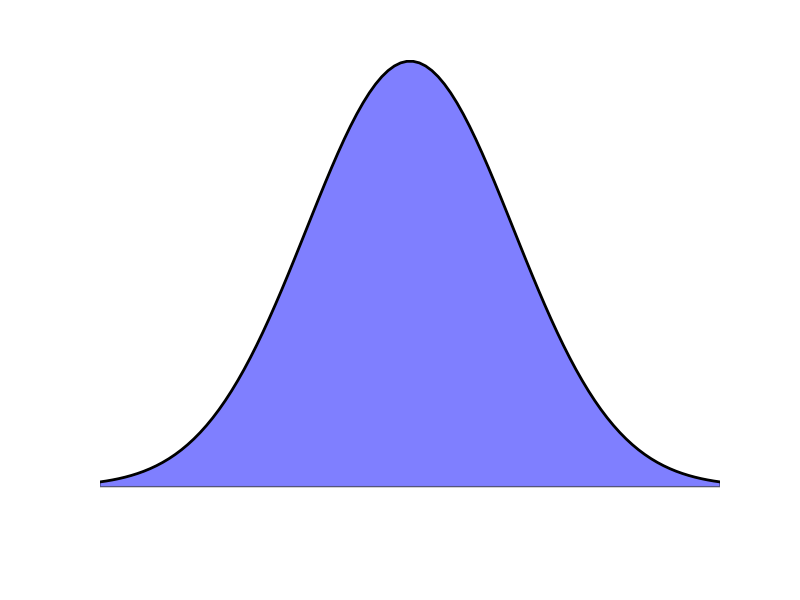
\includegraphics[width=.05\textwidth]{gaussian.png}};

    \node[inner sep=0cm] (gaussian) at (9.5,17.5)
        {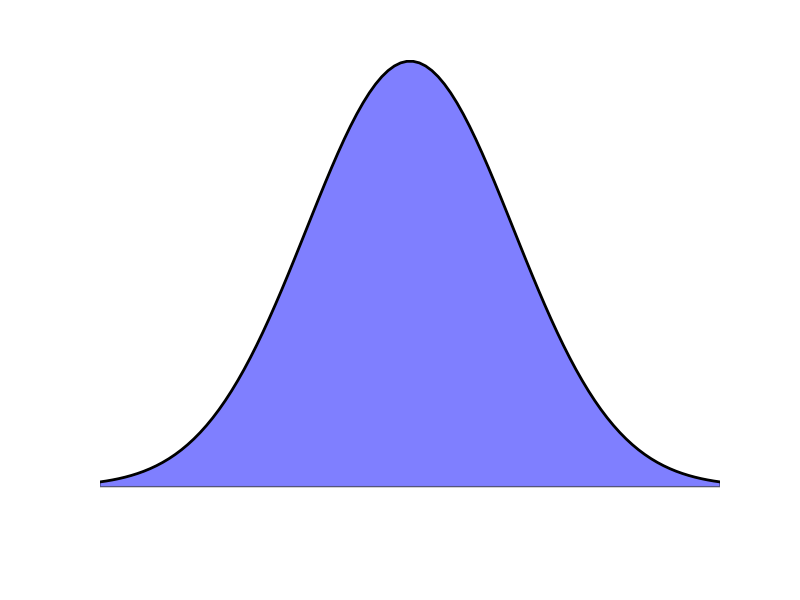
\includegraphics[width=.05\textwidth]{gaussian.png}};
    \node[inner sep=0cm] (gaussian) at (10.5,17.5)
        {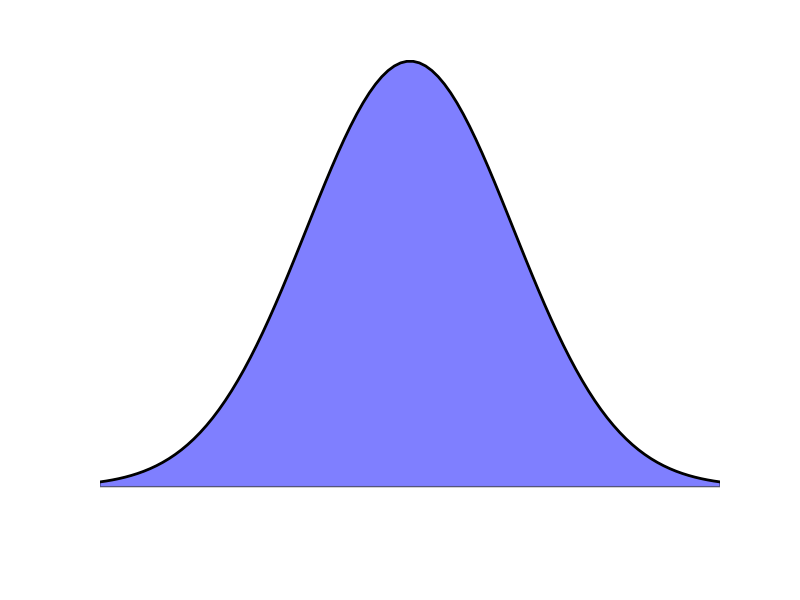
\includegraphics[width=.05\textwidth]{gaussian.png}};
    \node[inner sep=0cm] (gaussian) at (11.5,17.5)
        {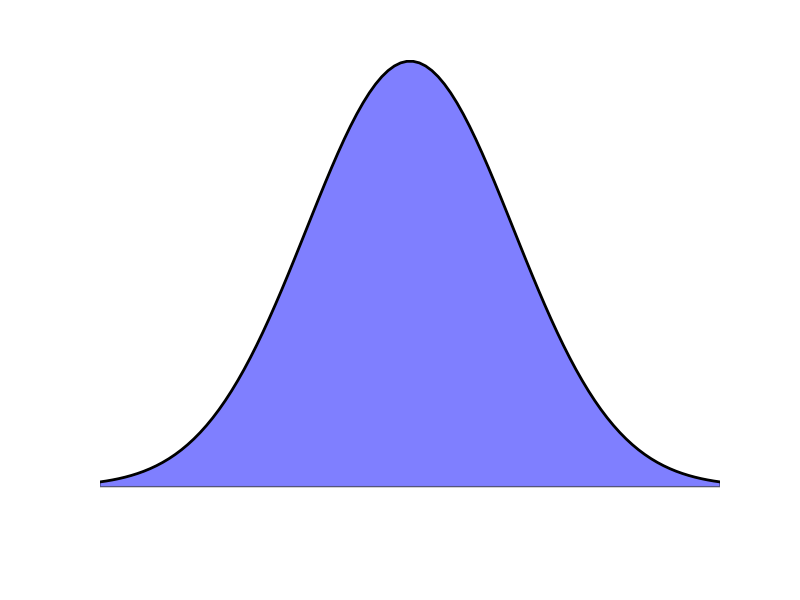
\includegraphics[width=.05\textwidth]{gaussian.png}};

    % First rectangle
    \draw (5,0) rectangle (8.5,3);
    \draw [fill=blue]   (5.5,1) rectangle (6,2);
    \draw [fill=green] (6.5,1) rectangle (7,2);
    \draw [fill=red]     (7.5,1) rectangle (8,2);

    % First gaussian filter
    \draw (1,6) rectangle (4.5,9);
    \draw (5,6) rectangle (8.5,9);
    \draw (9,6) rectangle (12.5,9);

    \draw [->,blue] (1.75,6) -- (2,5);
    \draw [->,blue] (2.75,6) -- (2.75,5.35);
    \draw [->,blue] (3.75,6) -- (3.5,5);
    \draw [->,blue] (2.75,4.5) -- (5,3);

    \draw [->,red] (9.75,6) -- (10,5);
    \draw [->,red] (10.75,6) -- (10.75,5.35);
    \draw [->,red] (11.75,6) -- (11.5,5);
    \draw [->,red] (10.75,4.5) -- (8.5,3);

    \draw [->,green] (5.75,6) -- (6,5);
    \draw [->,green] (6.75,6) -- (6.75,5.35);
    \draw [->,green] (7.75,6) -- (7.5,5);
    \draw [->,green] (6.75,4.5) -- (6.75,3);


    % middle rectangles 
    \draw (1,12) rectangle (4.5,15);
    \draw (5,12) rectangle (8.5,15);
    \draw (9,12) rectangle (12.5,15);

    \draw [fill=blue]   (1.5,13) rectangle (2,14);
    \draw [fill=blue]   (2.5,13) rectangle (3,14);
    \draw [fill=blue]   (3.5,13) rectangle (4,14);

    \draw [fill=green]   (5.5,13) rectangle (6,14);
    \draw [fill=green]   (6.5,13) rectangle (7,14);
    \draw [fill=green]   (7.5,13) rectangle (8,14);

    \draw [fill=red]   (9.5,13) rectangle (10,14);
    \draw [fill=red]   (10.5,13) rectangle (11,14);
    \draw [fill=red]   (11.5,13) rectangle (12,14);

    % small filter rectangles
    \draw (1,17) rectangle (2,18);
    \draw (2,17) rectangle (3,18);
    \draw (3,17) rectangle (4,18);

    \draw (5,17) rectangle (6,18);
    \draw (6,17) rectangle (7,18);
    \draw (7,17) rectangle (8,18);

    \draw (9,17) rectangle (10,18);
    \draw (10,17) rectangle (11,18);
    \draw (11,17) rectangle (12,18);

    % mult. rectangles and nodes
    \node at ( 2.75,10.5) [place] {$(*)$};
    \node at ( 6.75,10.5) [place] {$(*)$};
    \node at ( 10.75,10.5) [place] {$(*)$};

    \node at ( 2.75,19.5) [place] {$(*)$};
    \node at ( 6.75,19.5) [place] {$(*)$};
    \node at ( 10.75,19.5) [place] {$(*)$};

    % arrows of multiple rectangle nodes
    \draw [->,blue] (1.5,17) -- (1.5,15);
    \draw [->,blue] (5.5,17) -- (2.75,15);
    \draw [->,blue] (9.5,17) -- (3.75,15);

    \draw [->,green] (2.5,17) -- (5.5,15);
    \draw [->,green] (6.5,17) -- (6.75,15);
    \draw [->,green] (10.5,17) -- (7.75,15);

    \draw [->,red] (3.5,17) -- (9.5,15);
    \draw [->,red] (7.5,17) -- (10.75,15);
    \draw [->,red] (11.5,17) -- (11.75,15);

    % rectangles
    \draw (1,21) rectangle (4.5,24);
    \draw (5,21) rectangle (8.5,24);
    \draw (9,21) rectangle (12.5,24);

    \draw [fill=blue]   (1.5,22) rectangle (2,23);
    \draw [fill=green]   (2.5,22) rectangle (3,23);
    \draw [fill=red]   (3.5,22) rectangle (4,23);

    \draw [fill=blue]   (5.5,22) rectangle (6,23);
    \draw [fill=green]   (6.5,22) rectangle (7,23);
    \draw [fill=red]   (7.5,22) rectangle (8,23);

    \draw [fill=blue]   (9.5,22) rectangle (10,23);
    \draw [fill=green]   (10.5,22) rectangle (11,23);
    \draw [fill=red]   (11.5,22) rectangle (12,23);


    % sum nodes
    \node at ( 2.75,4.5) [place] {$\sum$};
    \node at ( 6.75,4.5) [place] {$\sum$};
    \node at ( 10.75,4.5) [place] {$\sum$};


\end{tikzpicture}
\end{document}
}
\fbox{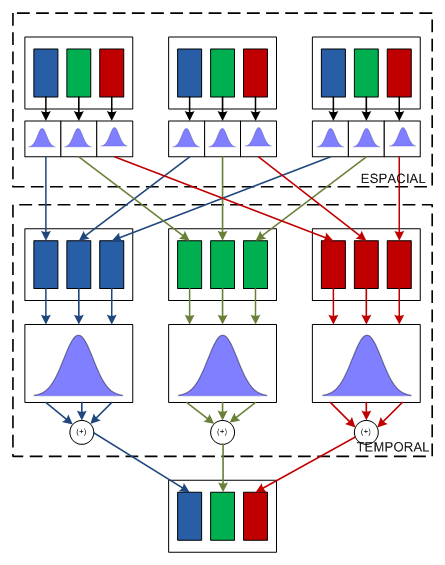
\includegraphics[scale=0.5]{img/Spatio_Temporal_Filter}}
\caption[Filtro temporal spacial]{Diagrama en bloques del filtro temporal y espacial. La parte de filtro temporal toma tres imágenes y aplica un filtro Gaussiano, el filtro espacial junta los componentes y aplica otro kernel Gaussiano.}
\label{fig:spatio_temporal_filter}
\end{figure}


Una representación en bloques de la implementación de este filtro se puede notar en la figura \ref{fig:spatio_temporal_filter}. La primera etapa es el procesamiento espacial, en que aplica un proceso de difuminado (\textit{blurring}) a cada uno de los colores de una imagen. Este procedimiento es un suavizado Gaussiano para reducir el ruido en la imagen de cada uno de los componentes. La segunda etapa consiste en agrupar por colores el resultado del filtrado espacial y luego utilizar un segundo filtro Gaussiano a cada uno de los tres componentes de las imágenes agrupadas por colores. El resultado es una suma de los tras componentes previamente filtrado. Finalmente, cada uno de los componentes se vuelven a juntar en una sola imagen con tres colores filtrados temporalmente.

\begin{figure}
\centering     %%% not \center
\subfigure[Resultado final sin filtro]{\label{fig:Figure_A}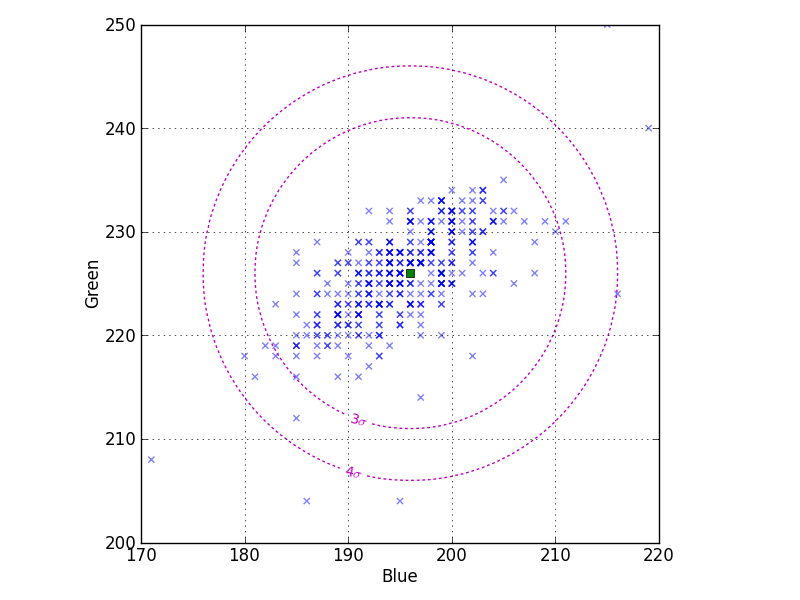
\includegraphics[width=100mm]{img/cluster_bg_340_160}}
\subfigure[Resultado final con filtro]{\label{fig:Figure_B}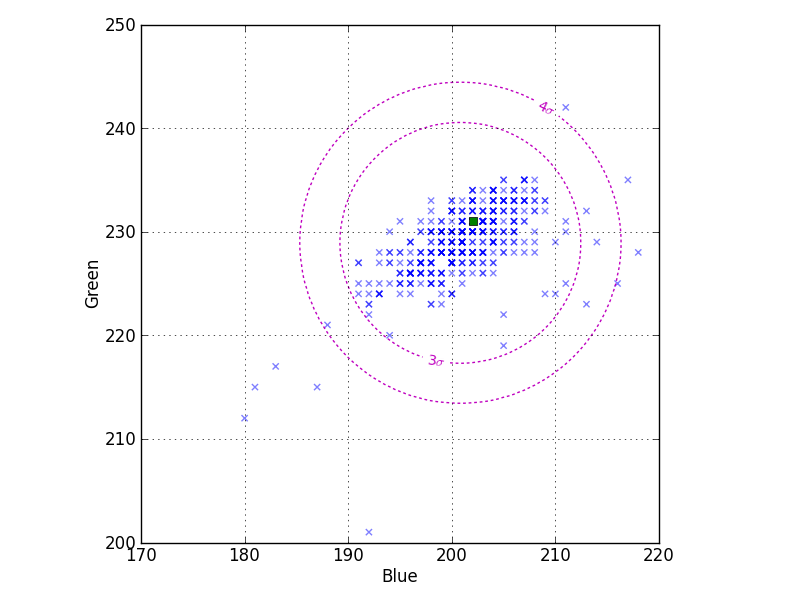
\includegraphics[width=100mm]{img/cluster_bg_340_160_filter}}
\caption[Comparación de efectividad del filtro en una secuencia completa]{Comparación de efectividad del filtro Espacial-Temporal aplicado en la secuencia completa }
\label{fig:result_spatio_temporal_filter}
\end{figure}


El efectividad de este filtro puede ser comparado en las figuras \ref{fig:result_spatio_temporal_filter}. La imagen \ref{fig:Figure_A} es el cluster de la imagen de fondo en funcionamiento normal del algoritmo sin filtro sobre las imágenes aplicado. En cambio la imagen de la figura \ref{fig:Figure_B} es el resultado final del cluster de la imagen de fondo,  aplicando procesamiento previo a las imágenes antes de ingresar en el algoritmo. Se puede observar que el cluster final filtrado es mucho más compacto que el otro. Finalmente esta de filtrado es una ayuda en el proceso de separación del fondo de imagen de los elementos móviles.



